\documentclass{beamer}

\usepackage{graphicx}
\usepackage{algorithm2e}
\usepackage{textpos}
\usepackage{etoolbox}
\usepackage{verbatim}

\setbeamertemplate{caption}[numbered]

\usepackage{tikz}
\usetikzlibrary{shapes.geometric}
\usetikzlibrary{arrows,shapes,trees}
\usetikzlibrary{calc,shapes.multipart,chains,arrows}
\usetikzlibrary{matrix,positioning}

\usepackage[dvipsnames]{xcolor}
\definecolor{pblue}{rgb}{0.13,0.13,1}
\definecolor{pgreen}{rgb}{0,0.5,0}
\definecolor{pred}{rgb}{0.9,0,0}
\definecolor{pgrey}{rgb}{0.46,0.45,0.48}

\usepackage{listings}
\lstset{language=Java,
    showspaces=false,
    showtabs=false,
    breaklines=true,
    showstringspaces=false,
    breakatwhitespace=true,
    commentstyle=\color{pgreen},
    keywordstyle=\color{pblue},
    stringstyle=\color{pred},
    basicstyle=\footnotesize,
    colframe=white!75!black,
    moredelim=[is][\textcolor{pgrey}]{\%\%}{\%\%}
}

\pgfdeclareshape{plain triangle}{
    \nodeparts{}
    \anchor{center}{\pgfpoint{0cm}{0cm}}
    \behindbackgroundpath{
		\path [draw,dashed] (0,0) -- (.5,-1) -- (-0.5,-1) -- cycle;
   }
   \pgfsetcolor{red}
}

\pgfdeclareshape{blue triangle}{
    \nodeparts{}
    \anchor{center}{\pgfpoint{0cm}{0cm}}
    \behindbackgroundpath{
		\path [draw,dashed, fill=blue] (0,0) -- (.5,-1) -- (-0.5,-1) -- cycle;
   }
   \pgfsetcolor{red}
}

\pgfdeclareshape{red triangle}{
    \nodeparts{}
    \anchor{center}{\pgfpoint{0cm}{0cm}}
    \behindbackgroundpath{
		\path [draw,dashed, fill=red] (0,0) -- (.5,-1) -- (-0.5,-1) -- cycle;
   }
   \pgfsetcolor{red}
}
\usetheme{Madrid}
\useoutertheme{miniframes} % Alternatively: miniframes, infolines, split



% Setup the university's color pallette
\definecolor{UIUCorange}{RGB}{19, 41, 75} % UBC Blue (primary)
\definecolor{UIUCblue}{RGB}{232, 74, 39} % UBC Grey (secondary)


\setbeamercolor{palette primary}{bg=UIUCorange,fg=white}
\setbeamercolor{palette secondary}{bg=UIUCblue,fg=white}
\setbeamercolor{palette tertiary}{bg=UIUCblue,fg=white}
\setbeamercolor{palette quaternary}{bg=UIUCblue,fg=white}
\setbeamercolor{structure}{fg=UIUCorange} % itemize, enumerate, etc
\setbeamercolor{section in toc}{fg=UIUCblue} % TOC sections

\setbeamercolor{subsection in head/foot}{bg=UIUCorange,fg=UIUCblue}
\setbeamercolor{subsection in head/foot}{bg=UIUCorange,fg=UIUCblue}

\usepackage[utf8]{inputenc}


%Information to be included in the title page:
\title{\textbf{Introduction to Graphs}}
\author{\textbf{David H Smith IV}}
\institute[\textbf{UIUC}]{\textbf{University of Illinois Urbana-Champaign}}
\date{\textbf{}}

\setbeamertemplate{title page}[default][colsep=-4bp,rounded=true]
\addtobeamertemplate{title page}{\vspace{3\baselineskip}}{}
\addtobeamertemplate{title page}{
    \begin{textblock*}{\paperwidth}(-1.0em, -1.2em)
        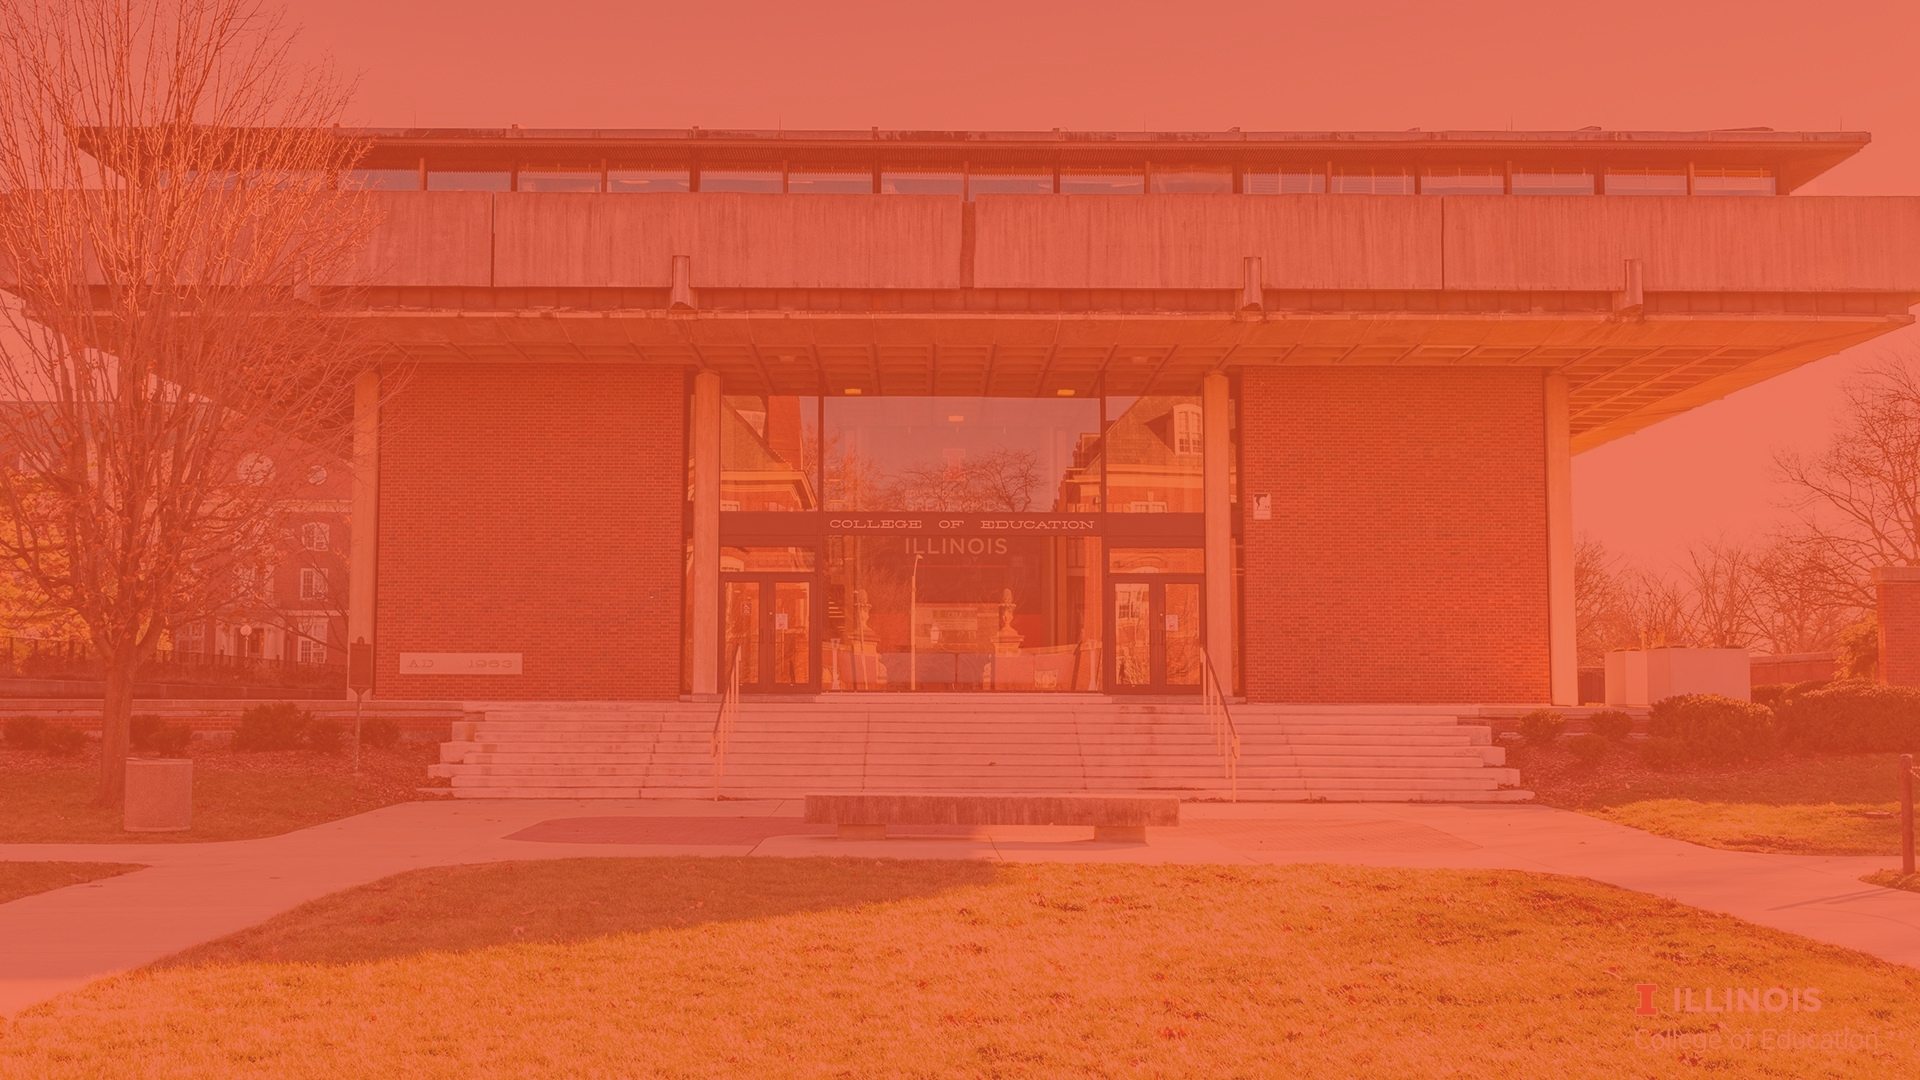
\includegraphics[width=\paperwidth, height=\paperheight]{imgs/uiuc.jpg}
    \end{textblock*} 
}{}

\begin{document}

\pgfdeclarelayer{background}
\pgfsetlayers{background,main}

\tikzstyle{vertex}=[circle,fill=black!25,minimum size=20pt,inner sep=0pt]
\tikzstyle{selected vertex} = [vertex, fill=orange!24]
\tikzstyle{edge} = [draw,thick,-]
\tikzstyle{weight} = [font=\small]
\tikzstyle{selected edge} = [draw,line width=5pt,-,blue!50]
\tikzstyle{ignored edge} = [draw,line width=5pt,-,black!20]


\frame{\titlepage}

\section{Objectives}
\begin{frame}
	\frametitle{Objectives}
    \centering
    \begin{itemize}
        \item Become familiar with graph terminology.
        \item How graphs are structured.
        \item How graphs are represented with adjacency matrices.
        \item Practice implementing some basic graph operations using adj matrices.
    \end{itemize}
\end{frame}

\begin{frame}
	\frametitle{Objectives}
    \centering
    \begin{itemize}
		\item \textbf{Week 10:} Introduction to graphs via Adj Matrices.
		\item \textbf{Week 11}: Introduction into Adj. Lists and Graphs Search Algorithms. Implementation 5 released.
		\item \textbf{Week 12}: Election day, checkpoint 1 due.
		\item \textbf{Week 13}: Shortest Path and Minimum Spanning Tree Algorithms. Implementation 5 due and 6 released.
		\item \textbf{Week 14}: Thanksgiving break.
		\item \textbf{Week 15}: Conclusion and Application 3 released. 
    \end{itemize}
\end{frame}

\section{Where we came from}
\begin{frame}[fragile]
	\frametitle{LinkedLists \textrightarrow Trees \textrightarrow Graphs}
    \begin{minipage}{0.32\textwidth}
		\centering
		\resizebox{\textwidth}{!}{
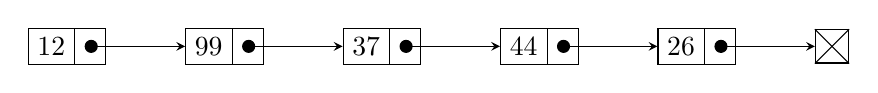
\begin{tikzpicture}[list/.style={rectangle split, rectangle split parts=2, draw, rectangle split horizontal}, >=stealth, start chain]

    \node[list,on chain] (A) {12};
    \node[list,on chain] (B) {99};
    \node[list,on chain] (D) {37};
    \node[list,on chain] (E) {44};
    \node[list,on chain] (F) {26};

    \node[on chain,draw,inner sep=6pt] (N) {};
    \draw (N.north east) -- (N.south west);
    \draw (N.north west) -- (N.south east);

    \draw[*->] let \p1 = (A.two), \p2 = (A.center) in (\x1,\y2) -- (B);
    \draw[*->] let \p1 = (B.two), \p2 = (B.center) in (\x1,\y2) -- (D);
    \draw[*->] let \p1 = (D.two), \p2 = (D.center) in (\x1,\y2) -- (E);
    \draw[*->] let \p1 = (E.two), \p2 = (E.center) in (\x1,\y2) -- (F);
    \draw[*->] let \p1 = (F.two), \p2 = (F.center) in (\x1,\y2) -- (N);


\end{tikzpicture}}\\


    \end{minipage}
    \begin{minipage}{0.32\textwidth}
		\centering
		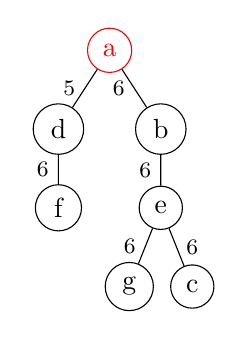
\begin{tikzpicture}[
    level distance = 1cm,
    level 1/.style = {sibling distance=1.3cm},
    level 2/.style = {sibling distance=1.0cm},
    level 3/.style = {sibling distance=0.8cm},
    every node/.style = {circle,draw},
    lbl/.style = {rectangle, draw=none, #1,% position
    font=\footnotesize}
    ]
    %
    \node (Root) [red] {a}
        child {node {d}
            child {node {f}
                edge from parent node[lbl=left] {$6$}
            }
            edge from parent node[lbl=left] {$5$}
        }
        child { node {b}
            child { node {e} 
                child{ 
                    node {g} 
                    edge from parent node[lbl=left] {$6$}
                }
                child{ 
                    node {c}
                    edge from parent node[lbl=right] {$6$}
                }
                edge from parent node[lbl=left] {$6$}
            }
            edge from parent node[lbl=left] {$6$}
        };
\end{tikzpicture}


    \end{minipage}
    \begin{minipage}{0.32\textwidth}
		\centering
		\begin{figure}[H]
\centering
\begin{tikzpicture}[scale=1.5, auto,swap]

    \foreach \pos/\name in {{(0,1)/a}, {(2,1)/b}, {(4,1)/c},
                            {(0,0)/d}, {(3,0)/e}, {(2,-1)/f}, {(4,-1)/g}}
        \node[vertex] (\name) at \pos {};

    \foreach \source/ \dest in {b/a, c/b,d/a,d/b,
                                         e/b,e/c,e/d,
                                         f/d,f/e,
                                         g/e,g/f}
        \draw[->, edge] (\source) -- (\dest);

\end{tikzpicture}
\end{figure}

    \end{minipage}
\end{frame}

\section{Graph Terms}
\begin{frame}[fragile]
	\frametitle{Terms}
    \centering
    \begin{minipage}{0.49\textwidth}
        \begin{figure}
            \begin{figure}[H]
\centering
\begin{tikzpicture}[scale=1.5]

    \foreach \pos/\name in {{(0,1)/a}, {(2,1)/b}, {(4,1)/c},
                            {(0,0)/d}, {(3,0)/e}, {(2,-1)/f}, {(4,-1)/g}}
        \node[vertex] (\name) at \pos {};

    \foreach \source/ \dest in {b/a/7, c/b/8,d/a/5,d/b/9,
                                         e/b/7, e/c/5,e/d/15,
                                         f/d/6,f/e/8,
                                         g/e/9,g/f/11}
        \draw[-{>},line width=0.9pt] (\source) to (\dest);
\end{tikzpicture}
\end{figure}





        \end{figure}
    \end{minipage}
\vfill
	\begin{itemize}
		\item \textbf{Vertex}: A ``Node'' in the graph.
		\item \textbf{Edge}: A connection between two vertecies.
        \item \textbf{Graph}: A set of edges ($E$) and a set of vertecies ($V$) and is often denoted as $G = (V, E)$.
	\end{itemize}
\end{frame}

\begin{frame}[fragile]
	\frametitle{Terms}
    \centering
    \begin{minipage}{0.49\textwidth}
        \begin{figure}
            \begin{figure}[H]
\centering
\begin{tikzpicture}[scale=1.5]

    \foreach \pos/\name in {{(0,1)/a}, {(2,1)/b}, {(4,1)/c},
                            {(0,0)/d}, {(3,0)/e}, {(2,-1)/f}, {(4,-1)/g}}
        \node[vertex] (\name) at \pos {};

    \foreach \source/ \dest in {b/a/7, c/b/8,d/a/5,d/b/9,
                                         e/b/7, e/c/5,e/d/15,
                                         f/d/6,f/e/8,
                                         g/e/9,g/f/11}
        \draw[-{>},line width=0.9pt] (\source) to (\dest);
\end{tikzpicture}
\end{figure}





        \end{figure}
    \end{minipage}
    \vfill
	\begin{itemize}
		\item \textbf{Directed v Undirected}: Can we move between vertecies in either direction or only in one? Examples of directed graphs include:
            \begin{itemize}
                \scriptsize
                \item \textbf{Linked Lists}: Once you move forward you cant move back.
                \item \textbf{Trees}: Once you proceed left you can \textit{directly} move back up to the parent.
            \end{itemize}
		\item \textbf{Weighted v Unweighted}: Does it cost us anything to move between vertecies?
	\end{itemize}
\end{frame}



\section{Types of Graphs}
\begin{frame}[fragile]
	\frametitle{Directed vs Undirected and Weighted vs Unweighted}
	\begin{minipage}{0.49\textwidth}
		\centering
		\begin{figure}[H]
\centering
\begin{tikzpicture}[scale=1.5, auto,swap]

    \foreach \pos/\name in {{(0,1)/a}, {(2,1)/b}, {(4,1)/c},
                            {(0,0)/d}, {(3,0)/e}, {(2,-1)/f}, {(4,-1)/g}}
        \node[vertex] (\name) at \pos {};

    \foreach \source/ \dest /\weight in {b/a/7, c/b/8,d/a/5,d/b/9,
                                         e/b/7, e/c/5,e/d/15,
                                         f/d/6,f/e/8,
                                         g/e/9,g/f/11}
        \draw[->, edge] (\source) -- node[weight] {$\weight$} (\dest);

\end{tikzpicture}
\end{figure}





		\textbf{Undirected, Weighted}
	\end{minipage}
	\hfill
	\begin{minipage}{0.49\textwidth}
		\centering
		\begin{figure}[H]
\centering
\begin{tikzpicture}[scale=1.5, auto,swap]

    \foreach \pos/\name in {{(0,1)/a}, {(2,1)/b}, {(4,1)/c},
                            {(0,0)/d}, {(3,0)/e}, {(2,-1)/f}, {(4,-1)/g}}
        \node[vertex] (\name) at \pos {};

    \foreach \source/ \dest in {b/a, c/b,d/a,d/b,
                                         e/b,e/c,e/d,
                                         f/d,f/e,
                                         g/e,g/f}
        \draw[->, edge] (\source) -- (\dest);

\end{tikzpicture}
\end{figure}

		\textbf{Undirected, Unweighted}
	\end{minipage}
	\vfill
	\begin{minipage}{0.49\textwidth}
		\centering
		\begin{figure}[H]
\centering
\begin{tikzpicture}[scale=1.5]

    \foreach \pos/\name in {{(0,1)/a}, {(2,1)/b}, {(4,1)/c},
                            {(0,0)/d}, {(3,0)/e}, {(2,-1)/f}, {(4,-1)/g}}
        \node[vertex] (\name) at \pos {};

    \foreach \source/ \dest in {b/a/7, c/b/8,d/a/5,d/b/9,
                                         e/b/7, e/c/5,e/d/15,
                                         f/d/6,f/e/8,
                                         g/e/9,g/f/11}
        \draw[-{>},line width=0.9pt] (\source) to (\dest);
\end{tikzpicture}
\end{figure}





		\textbf{Directed, Unweighted}
	\end{minipage}
	\hfill
	\begin{minipage}{0.49\textwidth}
		\centering
		\resizebox{0.75\textwidth}{!}{
\begin{tikzpicture}[scale=1.5, auto,swap]

    \foreach \pos/\name in {{(0,1)/a}, {(2,1)/b}, {(4,1)/c},
                            {(0,0)/d}, {(3,0)/e}, {(2,-1)/f}, {(4,-1)/g}}
        \node[vertex] (\name) at \pos {\name};

    \foreach \source/ \dest /\weight in {b/a/7, c/b/8,d/a/5,d/b/9,
                                         e/b/7, e/c/5,e/d/15,
                                         f/d/6,f/e/8,
                                         g/e/9,g/f/11}
        \draw[-{>},line width=0.9pt] (\source) -- node[weight] {$\weight$} (\dest);

\end{tikzpicture}}

		\textbf{Directed, Weighted}
	\end{minipage}
\end{frame}

\section{Graph Representations}

\begin{frame}
	\frametitle{Adjacency Matrix vs Adjacency List}
    \centering
	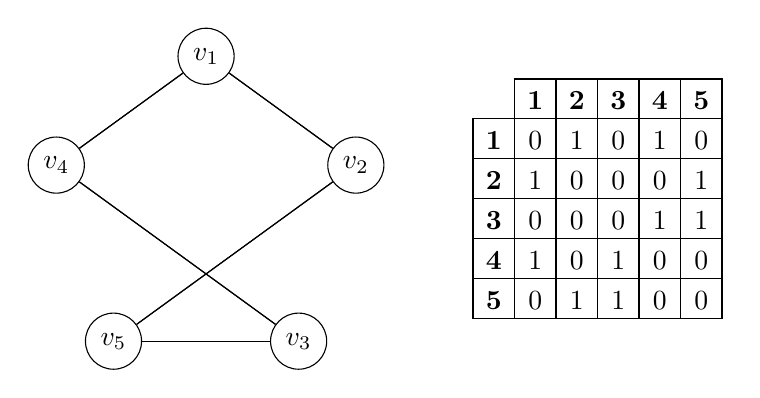
\begin{tikzpicture}[Bullet/.style={circle,draw,fill=black,inner sep=1.5pt},
		adjacency matrix/.style={ampersand replacement=\&,matrix of math nodes,
		row 1/.append style={nodes={font=\boldmath}},
		column 1/.append style={nodes={font=\boldmath}},nodes in empty cells,
		nodes={draw,minimum width=1.5em,text height=1.8ex},column sep=-\pgflinewidth,row
		sep=-\pgflinewidth}]

	\def\adjancymatrix{%
		{{0,1,0,1,0},%
		{1,0,0,0,1},%
		{0,0,0,1,1},%
		{1,0,1,0,0},%
		{0,1,1,0,0}}
    } 

	\let\mymatrixcontent\empty
	\def\mymatrixcontent{|[draw=none]|\& 1 \& 2 \& 3 \& 4 \& 5\\}
	\begin{scope}[local bounding box=right,xshift=10cm]
		\foreach \X in {1,...,3}
		{
			\node[draw, circle] (E\X) at (90+72-\X*72:2) {$v_\X$} ;
		}
		\node[draw, circle] (E5) at (90+72-4*72:2) {$v_5$} ; 
		\node[draw, circle] (E4) at (90+72-5*72:2) {$v_4$} ; 
		\foreach \X in {1,...,5}
		{\begingroup\edef\x{\endgroup
			\noexpand\gappto\noexpand\mymatrixcontent{\X }}\x
			\foreach \Y in {1,...,5}
			{\pgfmathtruncatemacro{\itest}{\adjancymatrix[\X-1][\Y-1]}
				\ifnum\itest=1
					\draw (E\X) -- (E\Y);
					\begingroup\edef\x{\endgroup
					\noexpand\gappto\noexpand\mymatrixcontent{\& \itest }}\x
				\else
					\begingroup\edef\x{\endgroup
					\noexpand\gappto\noexpand\mymatrixcontent{\& \itest }}\x
				\fi
			}
			\gappto\mymatrixcontent{\\}
		}
	\end{scope} 
	\matrix (rightmat) [right=of right,adjacency matrix]{
		\mymatrixcontent
	};
    \end{tikzpicture}
    \vfill
    \begin{enumerate}
        \item source vertex is the row.
        \item target vertex is the column.
        \item 1 for edge exist and 0 for it doesn't.
    \end{enumerate}
\end{frame}

\section{Adjacency Matrix}

\begin{frame}[fragile]
	\frametitle{Constructing Adj. Matrix - Unweighted, Undirected}
	\centering
	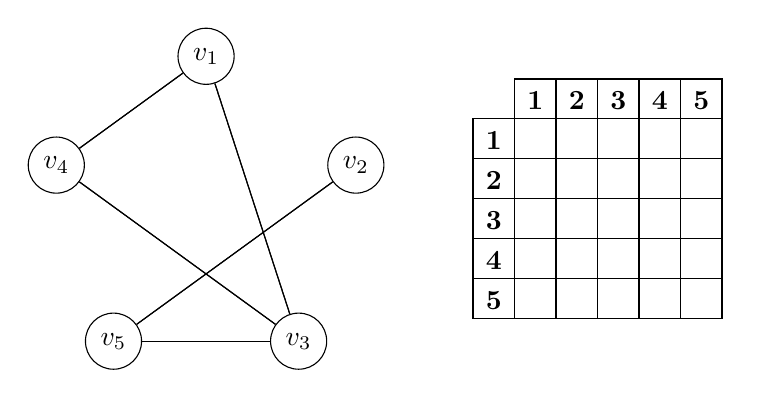
\begin{tikzpicture}[Bullet/.style={circle,draw,fill=black,inner sep=1.5pt},
		adjacency matrix/.style={ampersand replacement=\&,matrix of math nodes,
		row 1/.append style={nodes={font=\boldmath}},
		column 1/.append style={nodes={font=\boldmath}},nodes in empty cells,
		nodes={draw,minimum width=1.5em,text height=1.8ex},column sep=-\pgflinewidth,row
		sep=-\pgflinewidth}]

	\def\adjancymatrix{%
		{
            {0,0,1,1,0},%
            {0,0,0,0,1},%
            {1,0,0,1,1},%
            {1,0,1,0,0},%
            {0,1,1,0,0}
        }
    } 

	\let\mymatrixcontent\empty
	\def\mymatrixcontent{|[draw=none]|\& 1 \& 2 \& 3 \& 4 \& 5\\}
	\begin{scope}[local bounding box=right,xshift=10cm]
		\foreach \X in {1,...,3}
		{
			\node[draw, circle] (E\X) at (90+72-\X*72:2) {$v_\X$} ;
		}
		\node[draw, circle] (E5) at (90+72-4*72:2) {$v_5$} ; 
		\node[draw, circle] (E4) at (90+72-5*72:2) {$v_4$} ; 
		\foreach \X in {1,...,5}
		{\begingroup\edef\x{\endgroup
			\noexpand\gappto\noexpand\mymatrixcontent{\X }}\x
			\foreach \Y in {1,...,5}
			{\pgfmathtruncatemacro{\itest}{\adjancymatrix[\X-1][\Y-1]}
				\ifnum\itest=1
					\draw (E\X) -- (E\Y);
					\begingroup\edef\x{\endgroup
					\noexpand\gappto\noexpand\mymatrixcontent{\& }}\x
				\else
					\begingroup\edef\x{\endgroup
					\noexpand\gappto\noexpand\mymatrixcontent{\& }}\x
				\fi
			}
			\gappto\mymatrixcontent{\\}
		}
	\end{scope} 
	\matrix (rightmat) [right=of right,adjacency matrix]{
		\mymatrixcontent
	};
    \end{tikzpicture}
    \vfill
\end{frame}

\begin{frame}[fragile]
	\frametitle{Constructing Adj. Matrix - Weighted, Undirected}
	\centering
	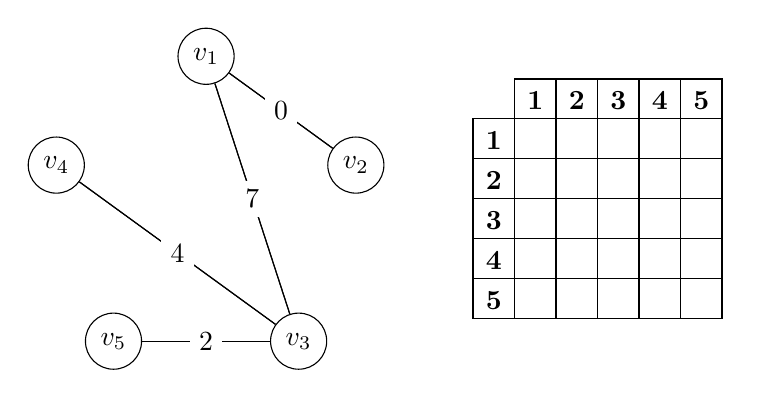
\begin{tikzpicture}[Bullet/.style={circle,draw,fill=black,inner sep=1.5pt},
		adjacency matrix/.style={ampersand replacement=\&,matrix of math nodes,
		row 1/.append style={nodes={font=\boldmath}},
		column 1/.append style={nodes={font=\boldmath}},nodes in empty cells,
		nodes={draw,minimum width=1.5em,text height=1.8ex},column sep=-\pgflinewidth,row
		sep=-\pgflinewidth}]

	\def\adjancymatrix{%
		{
            {-1,0,7,-1,-1},%
            {0,-1,-1,-1,-1},%
            {7,-1,-1,4,2},%
            {-1,-1,4,-1,-1},%
            {-1,-1,2,-1,-1}
        }
    } 

	\let\mymatrixcontent\empty
	\def\mymatrixcontent{|[draw=none]|\& 1 \& 2 \& 3 \& 4 \& 5\\}
	\begin{scope}[local bounding box=right,xshift=10cm]
		\foreach \X in {1,...,3}
		{
			\node[draw, circle] (E\X) at (90+72-\X*72:2) {$v_\X$} ;
		}
		\node[draw, circle] (E5) at (90+72-4*72:2) {$v_5$} ; 
		\node[draw, circle] (E4) at (90+72-5*72:2) {$v_4$} ; 
		\foreach \X in {1,...,5}
		{\begingroup\edef\x{\endgroup
			\noexpand\gappto\noexpand\mymatrixcontent{\X }}\x
			\foreach \Y in {1,...,5}
			{\pgfmathtruncatemacro{\itest}{\adjancymatrix[\X-1][\Y-1]}
                \ifnum\itest=-1
					\begingroup\edef\x{\endgroup
					\noexpand\gappto\noexpand\mymatrixcontent{\& }}\x
				\else
                    \path[-] (E\X) edge node[align=left, fill=white] {\itest} (E\Y);
					\begingroup\edef\x{\endgroup
					\noexpand\gappto\noexpand\mymatrixcontent{\& }}\x
				\fi
			}
			\gappto\mymatrixcontent{\\}
		}
	\end{scope} 
	\matrix (rightmat) [right=of right,adjacency matrix]{
		\mymatrixcontent
	};
    \end{tikzpicture}
    \vfill
\end{frame}

\begin{frame}[fragile]
	\frametitle{Constructing Adj. Matrix - Unweighted, Directed}
	\centering
	\centering
	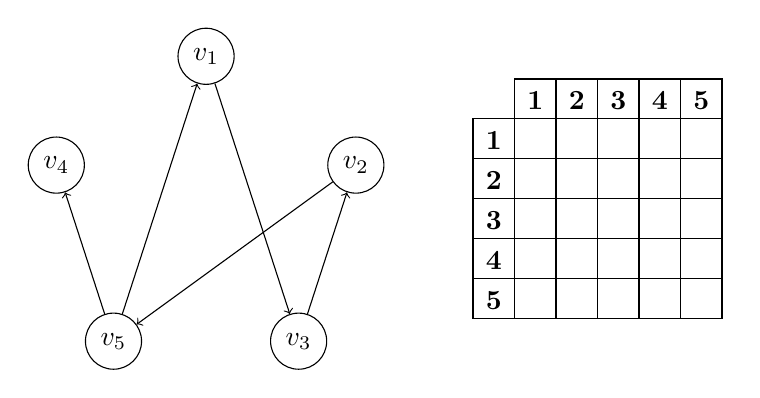
\begin{tikzpicture}[Bullet/.style={circle,draw,fill=black,inner sep=1.5pt},
		adjacency matrix/.style={ampersand replacement=\&,matrix of math nodes,
		row 1/.append style={nodes={font=\boldmath}},
		column 1/.append style={nodes={font=\boldmath}},nodes in empty cells,
		nodes={draw,minimum width=1.5em,text height=1.8ex},column sep=-\pgflinewidth,row
		sep=-\pgflinewidth}]

	\def\adjancymatrix{%
		{
            {0,0,1,0,0},%
            {0,0,0,0,1},%
            {0,1,0,0,0},%
            {0,0,0,0,0},%
            {1,0,0,1,0}
        }
    } 

	\let\mymatrixcontent\empty
	\def\mymatrixcontent{|[draw=none]|\& 1 \& 2 \& 3 \& 4 \& 5\\}
	\begin{scope}[local bounding box=right,xshift=10cm]
		\foreach \X in {1,...,3}
		{
			\node[draw, circle] (E\X) at (90+72-\X*72:2) {$v_\X$} ;
		}
		\node[draw, circle] (E5) at (90+72-4*72:2) {$v_5$} ; 
		\node[draw, circle] (E4) at (90+72-5*72:2) {$v_4$} ; 
		\foreach \X in {1,...,5}
		{\begingroup\edef\x{\endgroup
			\noexpand\gappto\noexpand\mymatrixcontent{\X }}\x
			\foreach \Y in {1,...,5}
			{\pgfmathtruncatemacro{\itest}{\adjancymatrix[\X-1][\Y-1]}
                \ifnum\itest=0
					\begingroup\edef\x{\endgroup
					\noexpand\gappto\noexpand\mymatrixcontent{\& }}\x
				\else
                    \path[->] (E\X) edge (E\Y);
					\begingroup\edef\x{\endgroup
					\noexpand\gappto\noexpand\mymatrixcontent{\& }}\x
				\fi
			}
			\gappto\mymatrixcontent{\\}
		}
	\end{scope} 
	\matrix (rightmat) [right=of right,adjacency matrix]{
		\mymatrixcontent
	};
    \end{tikzpicture}
    \vfill
\end{frame}

\begin{frame}[fragile]
	\frametitle{Constructing Adj. Matrix - Weighted, Undirected}
	\centering
	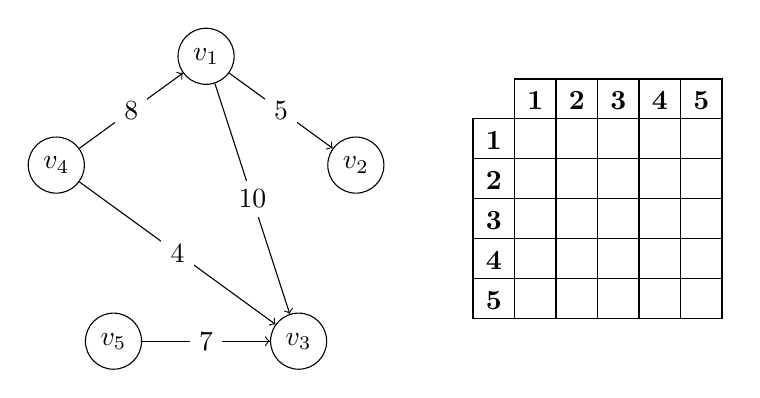
\begin{tikzpicture}[Bullet/.style={circle,draw,fill=black,inner sep=1.5pt},
		adjacency matrix/.style={ampersand replacement=\&,matrix of math nodes,
		row 1/.append style={nodes={font=\boldmath}},
		column 1/.append style={nodes={font=\boldmath}},nodes in empty cells,
		nodes={draw,minimum width=1.5em,text height=1.8ex},column sep=-\pgflinewidth,row
		sep=-\pgflinewidth}]

	\def\adjancymatrix{%
		{
            {0,5,10,0,0},%
            {0,0,0,0,0},%
            {0,0,0,0,0},%
            {8,0,4,0,0},%
            {0,0,7,0,0}
        }
    } 

	\let\mymatrixcontent\empty
	\def\mymatrixcontent{|[draw=none]|\& 1 \& 2 \& 3 \& 4 \& 5\\}
	\begin{scope}[local bounding box=right,xshift=10cm]
		\foreach \X in {1,...,3}
		{
			\node[draw, circle] (E\X) at (90+72-\X*72:2) {$v_\X$} ;
		}
		\node[draw, circle] (E5) at (90+72-4*72:2) {$v_5$} ; 
		\node[draw, circle] (E4) at (90+72-5*72:2) {$v_4$} ; 
		\foreach \X in {1,...,5}
		{\begingroup\edef\x{\endgroup
			\noexpand\gappto\noexpand\mymatrixcontent{\X }}\x
			\foreach \Y in {1,...,5}
			{\pgfmathtruncatemacro{\itest}{\adjancymatrix[\X-1][\Y-1]}
                \ifnum\itest=0
					\begingroup\edef\x{\endgroup
					\noexpand\gappto\noexpand\mymatrixcontent{\& }}\x
				\else
                    \path[->] (E\X) edge node[align=left, fill=white] {\itest} (E\Y);
					\begingroup\edef\x{\endgroup
					\noexpand\gappto\noexpand\mymatrixcontent{\& }}\x
				\fi
			}
			\gappto\mymatrixcontent{\\}
		}
	\end{scope} 
	\matrix (rightmat) [right=of right,adjacency matrix]{
		\mymatrixcontent
	};
    \end{tikzpicture}
    \vfill
\end{frame}

\begin{frame}[fragile]
    \frametitle{Adj Matrix - Practice}
    
    \begin{minipage}{0.24\textwidth}
        \resizebox{\textwidth}{!}{
        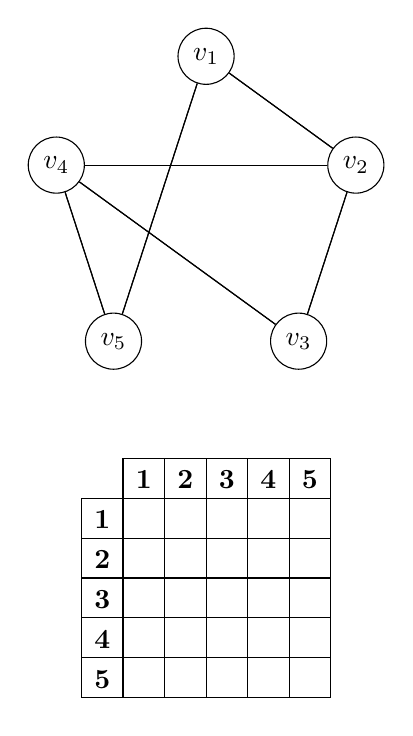
\begin{tikzpicture}[Bullet/.style={circle,draw,fill=black,inner sep=1.5pt},
            adjacency matrix/.style={ampersand replacement=\&,matrix of math nodes,
            row 1/.append style={nodes={font=\boldmath}},
            column 1/.append style={nodes={font=\boldmath}},nodes in empty cells,
            nodes={draw,minimum width=1.5em,text height=1.8ex},column sep=-\pgflinewidth,row
            sep=-\pgflinewidth}]

        \def\adjancymatrix{%
            {
                {0,1,0,0,1},%
                {1,0,1,1,0},%
                {0,1,0,1,0},%
                {0,1,1,0,1},%
                {1,0,0,1,0}
            }
        } 

        \let\mymatrixcontent\empty
        \def\mymatrixcontent{|[draw=none]|\& 1 \& 2 \& 3 \& 4 \& 5\\}
        \begin{scope}[local bounding box=right,xshift=10cm]
            \foreach \X in {1,...,3}
            {
                \node[draw, circle] (E\X) at (90+72-\X*72:2) {$v_\X$} ;
            }
            \node[draw, circle] (E5) at (90+72-4*72:2) {$v_5$} ; 
            \node[draw, circle] (E4) at (90+72-5*72:2) {$v_4$} ; 
            \foreach \X in {1,...,5}
            {\begingroup\edef\x{\endgroup
                \noexpand\gappto\noexpand\mymatrixcontent{\X }}\x
                \foreach \Y in {1,...,5}
                {\pgfmathtruncatemacro{\itest}{\adjancymatrix[\X-1][\Y-1]}
                    \ifnum\itest=0
                        \begingroup\edef\x{\endgroup
                        \noexpand\gappto\noexpand\mymatrixcontent{\& }}\x
                    \else
                        \path[-] (E\X) edge (E\Y);
                        \begingroup\edef\x{\endgroup
                        \noexpand\gappto\noexpand\mymatrixcontent{\& }}\x
                    \fi
                }
                \gappto\mymatrixcontent{\\}
            }
        \end{scope} 
        \matrix (rightmat) [below=of right,adjacency matrix]{
            \mymatrixcontent
        };
        \end{tikzpicture}}
    \end{minipage}
    \begin{minipage}{0.24\textwidth}
        \resizebox{\textwidth}{!}{
        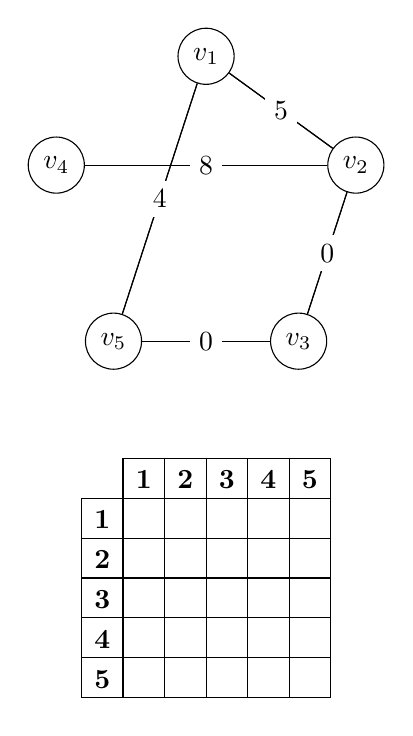
\begin{tikzpicture}[Bullet/.style={circle,draw,fill=black,inner sep=1.5pt},
            adjacency matrix/.style={ampersand replacement=\&,matrix of math nodes,
            row 1/.append style={nodes={font=\boldmath}},
            column 1/.append style={nodes={font=\boldmath}},nodes in empty cells,
            nodes={draw,minimum width=1.5em,text height=1.8ex},column sep=-\pgflinewidth,row
            sep=-\pgflinewidth}]

        \def\adjancymatrix{%
            {
                {-1,  5, -1, -1, 4}, %
                { 5, -1,  0,  8, -1}, %
                {-1,  0, -1, -1, 0}, %
                {-1,  8, -1, -1, -1}, %
                {4, -1, 0, -1, -1}
            }
        } 

        \let\mymatrixcontent\empty
        \def\mymatrixcontent{|[draw=none]|\& 1 \& 2 \& 3 \& 4 \& 5\\}
        \begin{scope}[local bounding box=right,xshift=10cm]
            \foreach \X in {1,...,3}
            {
                \node[draw, circle] (E\X) at (90+72-\X*72:2) {$v_\X$} ;
            }
            \node[draw, circle] (E5) at (90+72-4*72:2) {$v_5$} ; 
            \node[draw, circle] (E4) at (90+72-5*72:2) {$v_4$} ; 
            \foreach \X in {1,...,5}
            {\begingroup\edef\x{\endgroup
                \noexpand\gappto\noexpand\mymatrixcontent{\X }}\x
                \foreach \Y in {1,...,5}
                {\pgfmathtruncatemacro{\itest}{\adjancymatrix[\X-1][\Y-1]}
                    \ifnum\itest=-1
                        \begingroup\edef\x{\endgroup
                        \noexpand\gappto\noexpand\mymatrixcontent{\& }}\x
                    \else
                        \path[-] (E\X) edge node[align=left, fill=white] {\itest} (E\Y);
                        \begingroup\edef\x{\endgroup
                        \noexpand\gappto\noexpand\mymatrixcontent{\& }}\x
                    \fi
                }
                \gappto\mymatrixcontent{\\}
            }
        \end{scope} 
        \matrix (rightmat) [below=of right,adjacency matrix]{
            \mymatrixcontent
        };
        \end{tikzpicture}}
    \end{minipage}
    \begin{minipage}{0.24\textwidth}
        \resizebox{\textwidth}{!}{
        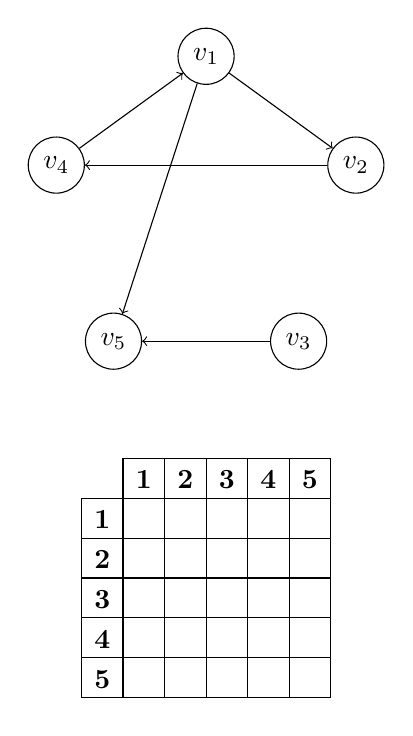
\begin{tikzpicture}[Bullet/.style={circle,draw,fill=black,inner sep=1.5pt},
            adjacency matrix/.style={ampersand replacement=\&,matrix of math nodes,
            row 1/.append style={nodes={font=\boldmath}},
            column 1/.append style={nodes={font=\boldmath}},nodes in empty cells,
            nodes={draw,minimum width=1.5em,text height=1.8ex},column sep=-\pgflinewidth,row
            sep=-\pgflinewidth}]

        \def\adjancymatrix{%
            {
                {0, 1, 0, 0, 1}, %
                {0, 0, 0, 1, 0}, %
                {0, 0, 0, 0, 1}, %
                {1, 0, 0, 0, 0}, %
                {0, 0, 0, 0, 0}
            }
        } 

        \let\mymatrixcontent\empty
        \def\mymatrixcontent{|[draw=none]|\& 1 \& 2 \& 3 \& 4 \& 5\\}
        \begin{scope}[local bounding box=right,xshift=10cm]
            \foreach \X in {1,...,3}
            {
                \node[draw, circle] (E\X) at (90+72-\X*72:2) {$v_\X$} ;
            }
            \node[draw, circle] (E5) at (90+72-4*72:2) {$v_5$} ; 
            \node[draw, circle] (E4) at (90+72-5*72:2) {$v_4$} ; 
            \foreach \X in {1,...,5}
            {\begingroup\edef\x{\endgroup
                \noexpand\gappto\noexpand\mymatrixcontent{\X }}\x
                \foreach \Y in {1,...,5}
                {\pgfmathtruncatemacro{\itest}{\adjancymatrix[\X-1][\Y-1]}
                    \ifnum\itest=0
                        \begingroup\edef\x{\endgroup
                        \noexpand\gappto\noexpand\mymatrixcontent{\& }}\x
                    \else
                        \path[->] (E\X) edge (E\Y);
                        \begingroup\edef\x{\endgroup
                        \noexpand\gappto\noexpand\mymatrixcontent{\& }}\x
                    \fi
                }
                \gappto\mymatrixcontent{\\}
            }
        \end{scope} 
        \matrix (rightmat) [below=of right,adjacency matrix]{
            \mymatrixcontent
        };
        \end{tikzpicture}}
    \end{minipage}
    \begin{minipage}{0.24\textwidth}
        \resizebox{\textwidth}{!}{
        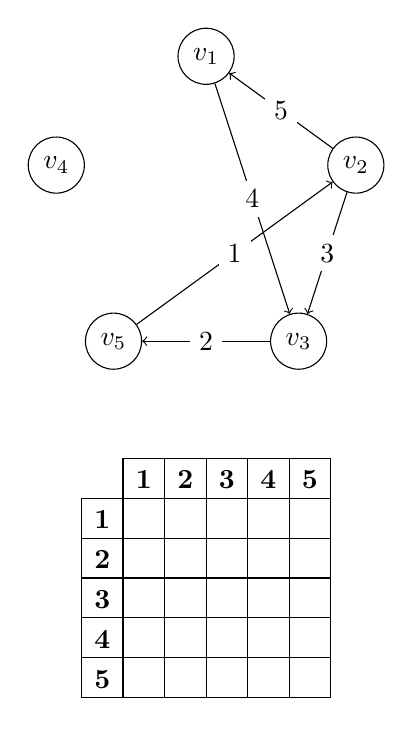
\begin{tikzpicture}[Bullet/.style={circle,draw,fill=black,inner sep=1.5pt},
            adjacency matrix/.style={ampersand replacement=\&,matrix of math nodes,
            row 1/.append style={nodes={font=\boldmath}},
            column 1/.append style={nodes={font=\boldmath}},nodes in empty cells,
            nodes={draw,minimum width=1.5em,text height=1.8ex},column sep=-\pgflinewidth,row
            sep=-\pgflinewidth}]

        \def\adjancymatrix{%
            {
                {0, 0, 4, 0,  0}, %
                {5, 0,  3, 0,  0}, %
                {0, 0,  0, 0,  2}, %
                {0, 0,  0, 0,  0}, %
                {0, 1,  0, 0,  0}
            }
        } 

        \let\mymatrixcontent\empty
        \def\mymatrixcontent{|[draw=none]|\& 1 \& 2 \& 3 \& 4 \& 5\\}
        \begin{scope}[local bounding box=right,xshift=10cm]
            \foreach \X in {1,...,3}
            {
                \node[draw, circle] (E\X) at (90+72-\X*72:2) {$v_\X$} ;
            }
            \node[draw, circle] (E5) at (90+72-4*72:2) {$v_5$} ; 
            \node[draw, circle] (E4) at (90+72-5*72:2) {$v_4$} ; 
            \foreach \X in {1,...,5}
            {\begingroup\edef\x{\endgroup
                \noexpand\gappto\noexpand\mymatrixcontent{\X }}\x
                \foreach \Y in {1,...,5}
                {\pgfmathtruncatemacro{\itest}{\adjancymatrix[\X-1][\Y-1]}
                    \ifnum\itest=0
                        \begingroup\edef\x{\endgroup
                        \noexpand\gappto\noexpand\mymatrixcontent{\& }}\x
                    \else
                        \draw[->] (E\X) edge node[align=left, fill=white, line width=2pt] {\itest} (E\Y);
                        \begingroup\edef\x{\endgroup
                        \noexpand\gappto\noexpand\mymatrixcontent{\& }}\x
                    \fi
                }
                \gappto\mymatrixcontent{\\}
            }
        \end{scope} 
        \matrix (rightmat) [below=of right,adjacency matrix]{
            \mymatrixcontent
        };
        \end{tikzpicture}}
    \end{minipage}
\end{frame}

\begin{frame}[fragile]
    \frametitle{Adj Matrix - Practice}
    
    \begin{minipage}{0.24\textwidth}
        \resizebox{\textwidth}{!}{
        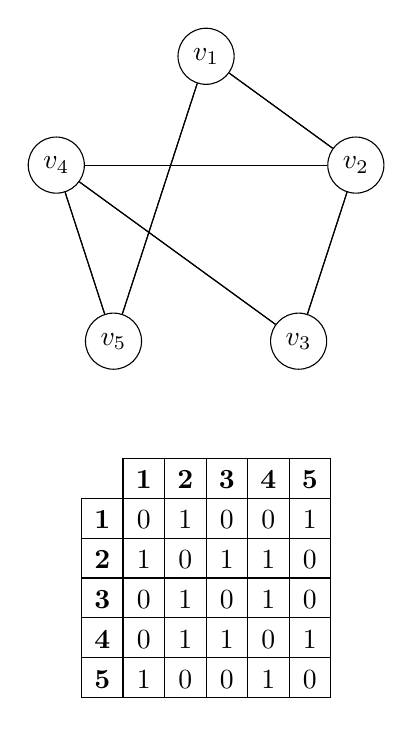
\begin{tikzpicture}[Bullet/.style={circle,draw,fill=black,inner sep=1.5pt},
            adjacency matrix/.style={ampersand replacement=\&,matrix of math nodes,
            row 1/.append style={nodes={font=\boldmath}},
            column 1/.append style={nodes={font=\boldmath}},nodes in empty cells,
            nodes={draw,minimum width=1.5em,text height=1.8ex},column sep=-\pgflinewidth,row
            sep=-\pgflinewidth}]

        \def\adjancymatrix{%
            {
                {0,1,0,0,1},%
                {1,0,1,1,0},%
                {0,1,0,1,0},%
                {0,1,1,0,1},%
                {1,0,0,1,0}
            }
        } 

        \let\mymatrixcontent\empty
        \def\mymatrixcontent{|[draw=none]|\& 1 \& 2 \& 3 \& 4 \& 5\\}
        \begin{scope}[local bounding box=right,xshift=10cm]
            \foreach \X in {1,...,3}
            {
                \node[draw, circle] (E\X) at (90+72-\X*72:2) {$v_\X$} ;
            }
            \node[draw, circle] (E5) at (90+72-4*72:2) {$v_5$} ; 
            \node[draw, circle] (E4) at (90+72-5*72:2) {$v_4$} ; 
            \foreach \X in {1,...,5}
            {\begingroup\edef\x{\endgroup
                \noexpand\gappto\noexpand\mymatrixcontent{\X }}\x
                \foreach \Y in {1,...,5}
                {\pgfmathtruncatemacro{\itest}{\adjancymatrix[\X-1][\Y-1]}
                    \ifnum\itest=0
                        \begingroup\edef\x{\endgroup
                        \noexpand\gappto\noexpand\mymatrixcontent{\& \itest}}\x
                    \else
                        \path[-] (E\X) edge (E\Y);
                        \begingroup\edef\x{\endgroup
                        \noexpand\gappto\noexpand\mymatrixcontent{\&  \itest}}\x
                    \fi
                }
                \gappto\mymatrixcontent{\\}
            }
        \end{scope} 
        \matrix (rightmat) [below=of right,adjacency matrix]{
            \mymatrixcontent
        };
        \end{tikzpicture}}
    \end{minipage}
    \begin{minipage}{0.24\textwidth}
        \resizebox{\textwidth}{!}{
        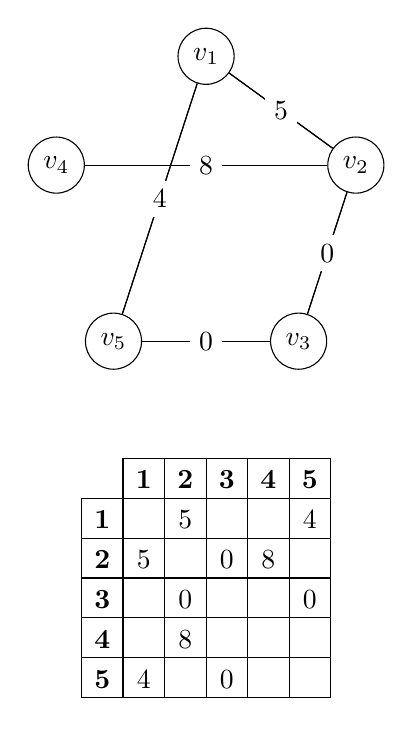
\begin{tikzpicture}[Bullet/.style={circle,draw,fill=black,inner sep=1.5pt},
            adjacency matrix/.style={ampersand replacement=\&,matrix of math nodes,
            row 1/.append style={nodes={font=\boldmath}},
            column 1/.append style={nodes={font=\boldmath}},nodes in empty cells,
            nodes={draw,minimum width=1.5em,text height=1.8ex},column sep=-\pgflinewidth,row
            sep=-\pgflinewidth}]

        \def\adjancymatrix{%
            {
                {-1,  5, -1, -1, 4}, %
                { 5, -1,  0,  8, -1}, %
                {-1,  0, -1, -1, 0}, %
                {-1,  8, -1, -1, -1}, %
                {4, -1, 0, -1, -1}
            }
        } 

        \let\mymatrixcontent\empty
        \def\mymatrixcontent{|[draw=none]|\& 1 \& 2 \& 3 \& 4 \& 5\\}
        \begin{scope}[local bounding box=right,xshift=10cm]
            \foreach \X in {1,...,3}
            {
                \node[draw, circle] (E\X) at (90+72-\X*72:2) {$v_\X$} ;
            }
            \node[draw, circle] (E5) at (90+72-4*72:2) {$v_5$} ; 
            \node[draw, circle] (E4) at (90+72-5*72:2) {$v_4$} ; 
            \foreach \X in {1,...,5}
            {\begingroup\edef\x{\endgroup
                \noexpand\gappto\noexpand\mymatrixcontent{\X }}\x
                \foreach \Y in {1,...,5}
                {\pgfmathtruncatemacro{\itest}{\adjancymatrix[\X-1][\Y-1]}
                    \ifnum\itest=-1
                        \begingroup\edef\x{\endgroup
                        \noexpand\gappto\noexpand\mymatrixcontent{\& }}\x
                    \else
                        \path[-] (E\X) edge node[align=left, fill=white] {\itest} (E\Y);
                        \begingroup\edef\x{\endgroup
                        \noexpand\gappto\noexpand\mymatrixcontent{\& \itest}}\x
                    \fi
                }
                \gappto\mymatrixcontent{\\}
            }
        \end{scope} 
        \matrix (rightmat) [below=of right,adjacency matrix]{
            \mymatrixcontent
        };
        \end{tikzpicture}}
    \end{minipage}
    \begin{minipage}{0.24\textwidth}
        \resizebox{\textwidth}{!}{
        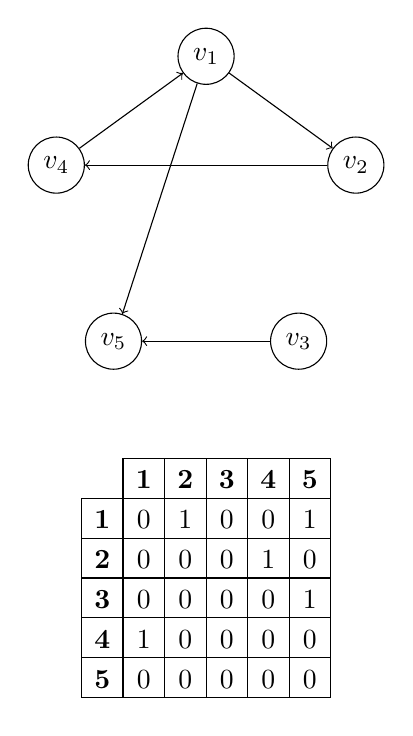
\begin{tikzpicture}[Bullet/.style={circle,draw,fill=black,inner sep=1.5pt},
            adjacency matrix/.style={ampersand replacement=\&,matrix of math nodes,
            row 1/.append style={nodes={font=\boldmath}},
            column 1/.append style={nodes={font=\boldmath}},nodes in empty cells,
            nodes={draw,minimum width=1.5em,text height=1.8ex},column sep=-\pgflinewidth,row
            sep=-\pgflinewidth}]

        \def\adjancymatrix{%
            {
                {0, 1, 0, 0, 1}, %
                {0, 0, 0, 1, 0}, %
                {0, 0, 0, 0, 1}, %
                {1, 0, 0, 0, 0}, %
                {0, 0, 0, 0, 0}
            }
        } 

        \let\mymatrixcontent\empty
        \def\mymatrixcontent{|[draw=none]|\& 1 \& 2 \& 3 \& 4 \& 5\\}
        \begin{scope}[local bounding box=right,xshift=10cm]
            \foreach \X in {1,...,3}
            {
                \node[draw, circle] (E\X) at (90+72-\X*72:2) {$v_\X$} ;
            }
            \node[draw, circle] (E5) at (90+72-4*72:2) {$v_5$} ; 
            \node[draw, circle] (E4) at (90+72-5*72:2) {$v_4$} ; 
            \foreach \X in {1,...,5}
            {\begingroup\edef\x{\endgroup
                \noexpand\gappto\noexpand\mymatrixcontent{\X }}\x
                \foreach \Y in {1,...,5}
                {\pgfmathtruncatemacro{\itest}{\adjancymatrix[\X-1][\Y-1]}
                    \ifnum\itest=0
                        \begingroup\edef\x{\endgroup
                        \noexpand\gappto\noexpand\mymatrixcontent{\& \itest}}\x
                    \else
                        \path[->] (E\X) edge (E\Y);
                        \begingroup\edef\x{\endgroup
                        \noexpand\gappto\noexpand\mymatrixcontent{\& \itest}}\x
                    \fi
                }
                \gappto\mymatrixcontent{\\}
            }
        \end{scope} 
        \matrix (rightmat) [below=of right,adjacency matrix]{
            \mymatrixcontent
        };
        \end{tikzpicture}}
    \end{minipage}
    \begin{minipage}{0.24\textwidth}
        \resizebox{\textwidth}{!}{
        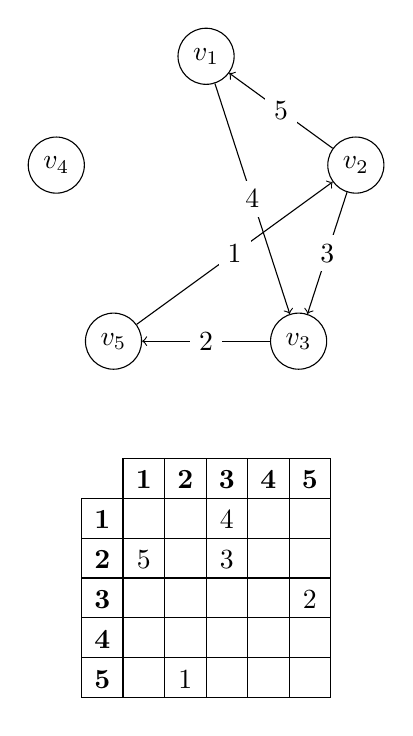
\begin{tikzpicture}[Bullet/.style={circle,draw,fill=black,inner sep=1.5pt},
            adjacency matrix/.style={ampersand replacement=\&,matrix of math nodes,
            row 1/.append style={nodes={font=\boldmath}},
            column 1/.append style={nodes={font=\boldmath}},nodes in empty cells,
            nodes={draw,minimum width=1.5em,text height=1.8ex},column sep=-\pgflinewidth,row
            sep=-\pgflinewidth}]

        \def\adjancymatrix{%
            {
                {0, 0, 4, 0,  0}, %
                {5, 0,  3, 0,  0}, %
                {0, 0,  0, 0,  2}, %
                {0, 0,  0, 0,  0}, %
                {0, 1,  0, 0,  0}
            }
        } 

        \let\mymatrixcontent\empty
        \def\mymatrixcontent{|[draw=none]|\& 1 \& 2 \& 3 \& 4 \& 5\\}
        \begin{scope}[local bounding box=right,xshift=10cm]
            \foreach \X in {1,...,3}
            {
                \node[draw, circle] (E\X) at (90+72-\X*72:2) {$v_\X$} ;
            }
            \node[draw, circle] (E5) at (90+72-4*72:2) {$v_5$} ; 
            \node[draw, circle] (E4) at (90+72-5*72:2) {$v_4$} ; 
            \foreach \X in {1,...,5}
            {\begingroup\edef\x{\endgroup
                \noexpand\gappto\noexpand\mymatrixcontent{\X }}\x
                \foreach \Y in {1,...,5}
                {\pgfmathtruncatemacro{\itest}{\adjancymatrix[\X-1][\Y-1]}
                    \ifnum\itest=0
                        \begingroup\edef\x{\endgroup
                        \noexpand\gappto\noexpand\mymatrixcontent{\& }}\x
                    \else
                        \draw[->] (E\X) edge node[align=left, fill=white, line width=2pt] {\itest} (E\Y);
                        \begingroup\edef\x{\endgroup
                        \noexpand\gappto\noexpand\mymatrixcontent{\& \itest}}\x
                    \fi
                }
                \gappto\mymatrixcontent{\\}
            }
        \end{scope} 
        \matrix (rightmat) [below=of right,adjacency matrix]{
            \mymatrixcontent
        };
        \end{tikzpicture}}
    \end{minipage}
\end{frame}


\section{Adj. Matrix - Java}
\begin{frame}[fragile]
    \frametitle{Adj Matrix - Vertex Count and Edge List to Adj Matrix}
    \begin{lstlisting}[basicstyle=\scriptsize, frame=trBL]
public void printAdjMatrix(List<Integer[]> edges, int vertexCount){
    //Step 1: Create a NxN matrix 
    int[][] matrix = ??
    
    //Step 2: Populate the matrix using vertex list
    for(Integer[] pair: edges){
        
    }
    //Step 3: Print the matrix 
}
    \end{lstlisting}
    \begin{enumerate}
		\scriptsize
        \item \textbf{Input:} Vertex count and list of edges
        \item Steps:
            \begin{itemize}
				\scriptsize
                \item Step 1: Initialize the 2d Array to be an NxN matrix where N is the vertex count.
                \item Step 2: Iterate over the list of edges (source, target) and set 
                    \begin{itemize}
						\tiny
                        \item Recall that target is the row and source is the column
                    \end{itemize}
                \item Step 3: Iterate over the matrix in order to display its contents.
            \end{itemize}
    \end{enumerate}
\end{frame}

\begin{frame}[fragile]
    \frametitle{Adj Matrix - Class}
    \begin{lstlisting}[basicstyle=\scriptsize, frame=trBL]
class MatrixGraph {
    private Integer[][] graph;
    private boolean isDirected;
    
    // Step 1: Initialize an NxN graph with all 0s
    MatrixGraph(int numVertecies, boolean isDirected){ ... }
    
    //Step 2: Construct an AddEdge Method
    public void addEdge(int v1, int v2, int edgeWeight){ ... }
} 
    \end{lstlisting}
    \begin{enumerate}
		\scriptsize
        \item \textbf{Step 1 - Constructor:} The constructor should take a \lstinline|vertexCount| and an \lstinline|isDirected|. It should initialize the graph to be an NxN array and populate it 
        \item \textbf{Step 2 - Add Edge:} This method should add populate the cell are the row/column as specified by the source/target. If isDirected is false, it should also add the edge going in the other direction.
    \end{enumerate}
\end{frame}

\end{document}
